\section{Resultados}\label{sec:results}

\begin{table}[H]
\centering
\footnotesize
\setlength{\tabcolsep}{4pt}
\renewcommand{\arraystretch}{1.25}
\begin{tabularx}{\textwidth}{@{}>{\raggedright\arraybackslash}p{5.7cm}>{\raggedright\arraybackslash}p{3.8cm}>{\raggedright\arraybackslash}X@{}}
\toprule
Classifier & Key settings & Five-fold CV result(s) \\
\midrule
\var{DecisionTreeClassifier} &
CART con Gini; profundidad máxima 3, mínimo de 500 observaciones por hoja, umbral 0,25. &
ROC-AUC: $0{,}7372 \pm 0{,}0044$ \newline
Exactitud equilibrada: $0{,}6732 \pm 0{,}0067$ \newline
F1: $0{,}4846 \pm 0{,}0107$ \newline
Exactitud: $0{,}7793 \pm 0{,}0090$ \newline
Sensibilidad: $0{,}4890 \pm 0{,}0073$ \newline
Precisión: $0{,}4805 \pm 0{,}0164$ \\
\addlinespace
\var{LogisticRegression} &
Penalización L1, $C \in \{0{,}1; 1; 10\}$, 19 columnas transformada,2 umbral 0,20 o 0,25. &
ROC-AUC: $0{,}7515 \pm 0{,}0075$ \newline
Exactitud equilibrada: $0{,}6806 \pm 0{,}0044$ \newline
F1: $0{,}4833 \pm 0{,}0035$ \newline
Exactitud: $0{,}7297 \pm 0{,}0316$ \newline
Sensibilidad: $0{,}5955 \pm 0{,}0627$ \newline
Precisión: $0{,}4109 \pm 0{,}0305$ \\
\addlinespace
\var{ExplainableBoostingClassifier} &
15 funciones univariantes, interactions=0, \var{max_bins}=32, mínimo de 10 observaciones por hoja, umbral 0,20 o 0,25. &
ROC-AUC: $0{,}7755 \pm 0{,}0077$ \newline
Exactitud equilibrada: $0{,}6997 \pm 0{,}0064$ \newline
F1: $0{,}5068 \pm 0{,}0105$ \newline
Exactitud: $0{,}7342 \pm 0{,}0367$ \newline
Sensibilidad: $0{,}6405 \pm 0{,}0531$ \newline
Precisión: $0{,}4232 \pm 0{,}0380$ \\
\bottomrule
\end{tabularx}
\caption{Resultados de las tres familias con el umbral interno seleccionado en cada partición. Todas las métricas se expresan como media $\pm$ desviación típica de las cinco particiones externas. Clase positiva = 1.}
\label{tab:results}
\end{table}

La Tabla~\ref{tab:results} resume los resultados de las tres familias con los umbrales internos; las subsecciones siguientes detallan la configuración seleccionada y el comportamiento observado.

\subsection{Árbol de decisión}

El árbol seleccionó en las cinco particiones una profundidad máxima de 3 y un mínimo de 500 observaciones por hoja, con umbral 0,25. La estructura resultante tiene 8 hojas y 15 nodos, emplea entre 3 y 5 variables transformadas y la primera división se guía según \var{latest_repayment_status}. Su ROC-AUC externa fue $0{,}7372 \pm 0{,}0044$, la más baja de las tres familias. El diagnóstico sin restricciones mostró una ROC-AUC de entrenamiento próxima a 1 frente a $0{,}5985$ en validación, con profundidades de 37 a 54 y evidencia de sobreajuste.

\subsection{Regresión logística}

La regresión logística seleccionó penalización L1 en las cinco particiones, con valores de $C$ entre 0,1 y 10 y umbrales de 0,20 o 0,25. El valor de $C$ fue 0,1 en dos particiones, 1 en dos y 10 en una. Retuvo entre 15 y 19 coeficientes no nulos sobre 19 columnas transformadas, correspondientes a 14 o 15 variables originales. Su ROC-AUC externa fue $0{,}7515 \pm 0{,}0075$. Con el umbral interno obtuvo una exactitud de $0{,}7297$, una exactitud equilibrada de $0{,}6806$ y una sensibilidad de $0{,}5955$.

\subsection{EBM}

El EBM sin interacciones seleccionó \var{max_bins}=32 en las cinco particiones y un mínimo de 10 observaciones por hoja en cuatro de ellas (50 en la restante), con umbrales de 0,20 o 0,25. El modelo comparado emplea 15 funciones univariantes. Alcanzó la mayor ROC-AUC externa ($0{,}7755 \pm 0{,}0077$) y, con el umbral interno, la mayor exactitud equilibrada ($0{,}6997$), sensibilidad ($0{,}6405$) y F1 ($0{,}5068$); su exactitud fue $0{,}7342$.

\subsection{Efecto del umbral y errores}

\begin{table}[H]
\centering
\footnotesize
\begin{tabular}{@{}lrrrr@{}}
\toprule
Classifier & Exactitud & Exactitud equilibrada & Sensibilidad & Precisión \\
\midrule
\var{DecisionTreeClassifier} & $-2{,}46$ & $+11{,}07$ & $+34{,}59$ & $-20{,}06$ \\
\var{LogisticRegression} & $-8{,}09$ & $+7{,}70$ & $+35{,}14$ & $-22{,}94$ \\
\var{ExplainableBoostingClassifier} & $-8{,}36$ & $+7{,}18$ & $+34{,}23$ & $-23{,}25$ \\
\bottomrule
\end{tabular}
\caption{Cambio medio al pasar del umbral 0,5 al umbral interno, en puntos porcentuales (calculado antes de redondear; cinco particiones externas; clase positiva = 1).}
\label{tab:threshold}
\end{table}

La Tabla~\ref{tab:threshold} muestra el cambio medio al sustituir el umbral 0,5 por el umbral interno. En las tres familias la exactitud disminuye entre 2,46 y 8,36 puntos porcentuales, mientras que la sensibilidad aumenta más de 34 puntos y la precisión cae más de 20. La exactitud equilibrada mejora 11,07 puntos en el árbol, 7,70 en la logística y 7,18 en el EBM. Con 0,5 los tres modelos superaban la exactitud mayoritaria, pero detectaban menos del 30\,\% de los positivos.

Las matrices de confusión de las predicciones fuera de muestra (OOF) con umbral interno (Figura~\ref{fig:confusion}) registran 2\,593 verdaderos positivos y 2\,710 falsos negativos en el árbol, 3\,159 y 2\,144 en la logística, y 3\,401 y 1\,902 en el EBM. Respecto a la logística, el EBM añade 242 verdaderos positivos y 130 falsos positivos; respecto al árbol, 808 verdaderos positivos y 1\,936 falsos positivos. Al bajar el umbral, el EBM incorpora 1\,820 verdaderos positivos y 3\,909 falsos positivos. Los tres coinciden en 16\,056 aciertos y 3\,833 fallos, de los que 1\,634 son positivos (30,81\,\% de los positivos). La exactitud con umbral interno queda por debajo de la referencia mayoritaria (0,7879) en los tres casos.

\begin{figure}[H]
	\centering
	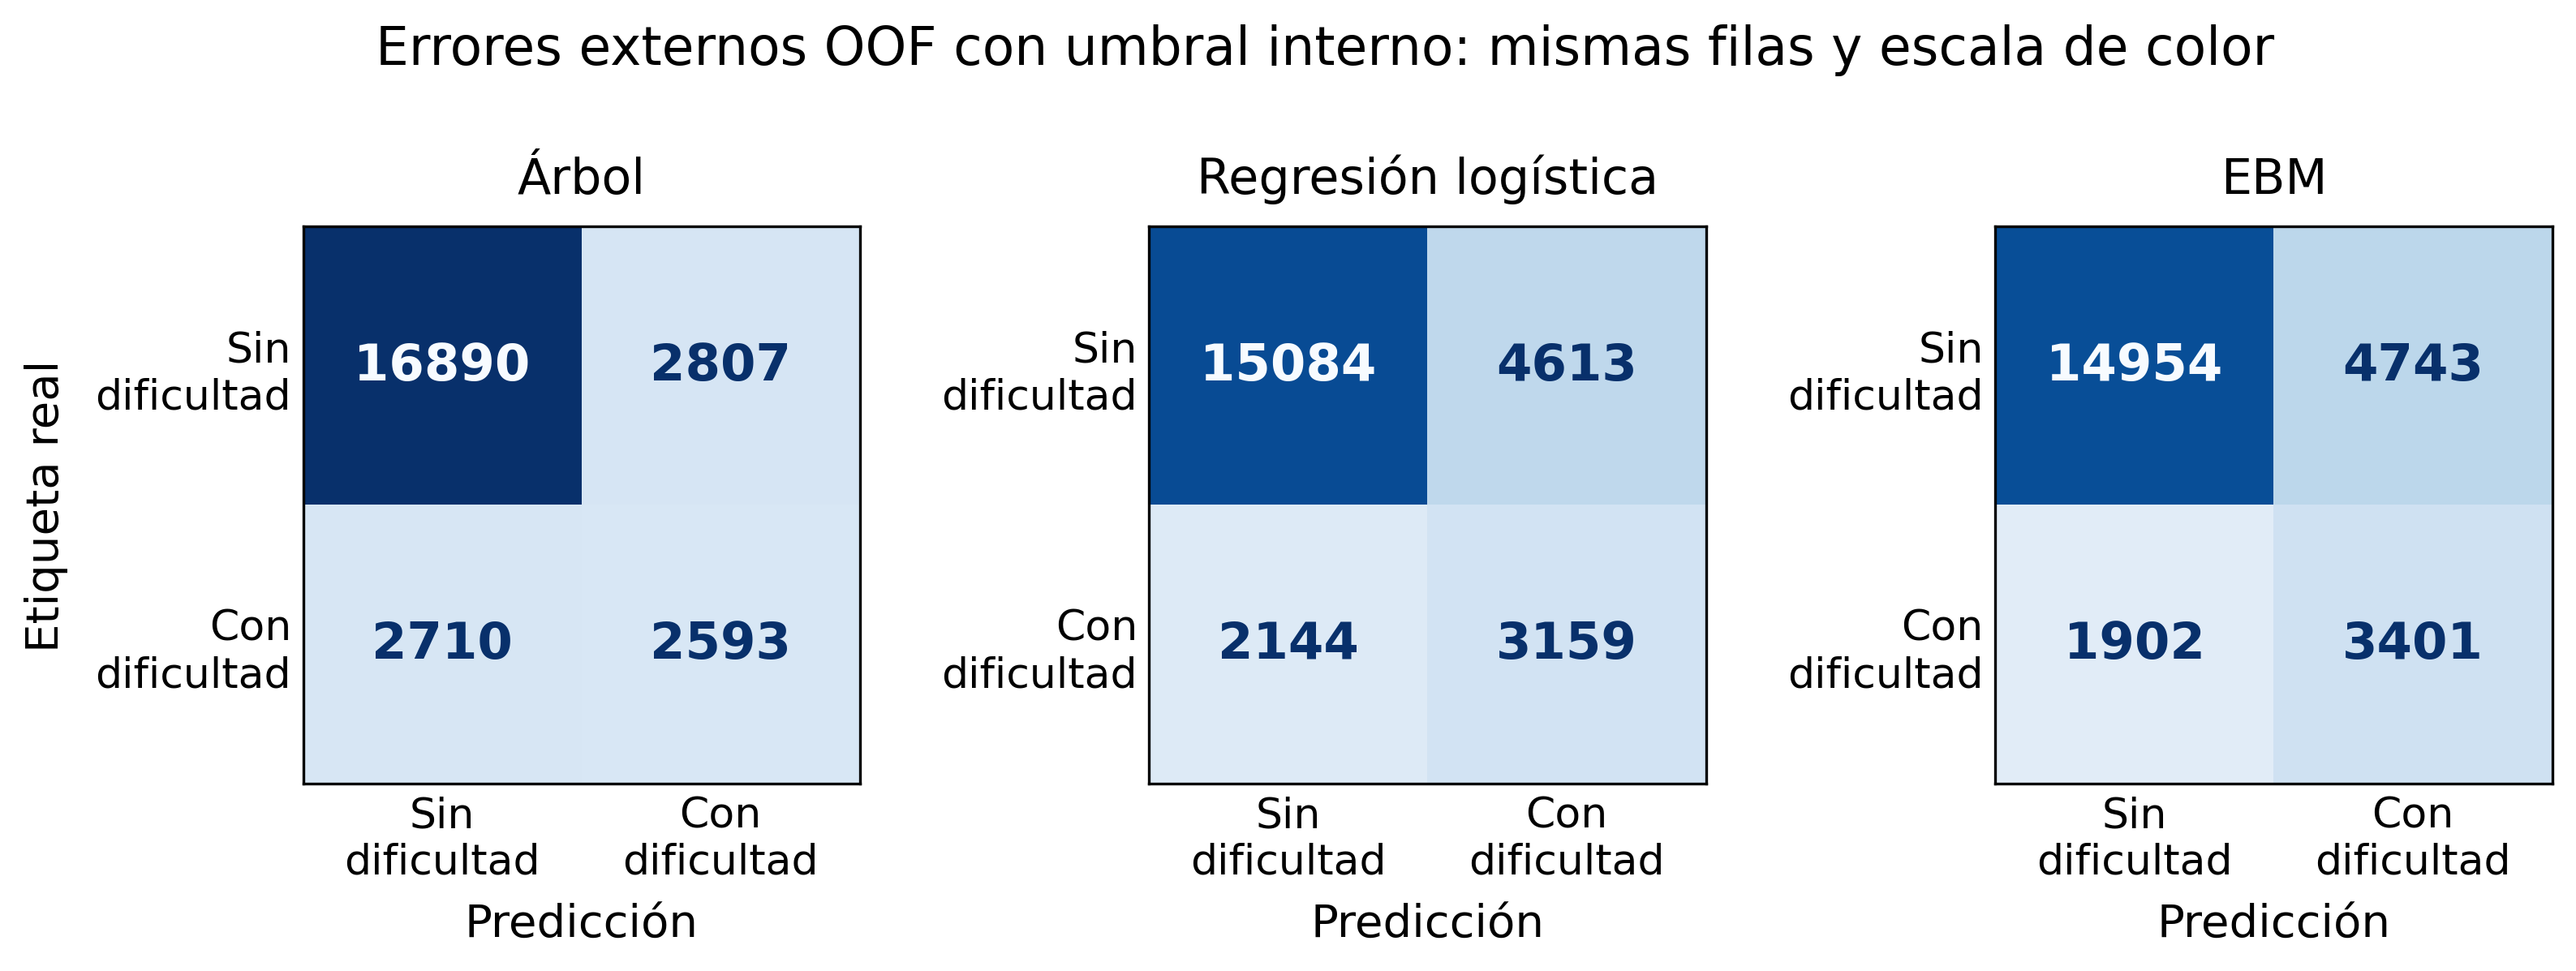
\includegraphics[width=\textwidth]{images/phase2_confusion_matrices.png}
	\caption{Matrices de confusión de los tres modelos con umbral interno. Filas: clase real; columnas: clase predicha; la escala de color es común a los tres paneles.}
	\label{fig:confusion}
\end{figure}
